\section{Components i Característiques TX/RX}
A continuació es descriuen els dos tipus de altímetres segons la seva modulació:
\subsection{Altimetre basat en modulació per freqüència FMCW}
Utilitza dues antenes, una per l'emissió (TX) i una per la recepció(RX). La senyal emesa rebota al terra i retorna a l'aeronau. Durant tota l'estona, el sistema de transmissió va variant la freqüència dins d'un rang, típicament de 50MHz. Així, quan arriba la senyal rebotada, existeix una $\Delta f$ entre aquesta i la senyal TX. Coneixent la velocitat de variació de la freqüència d'emissió $\frac{df}{dt}$ es pot deduir l'alçada $H$ de l'aeronau. Cal remarcar que el sistema omet els efectes Doppler degut a que són despreciables en comparació amb l'efecte de la variació de la freqüència de la modulació FMCW.
\begin{figure}[H]
	\centering
	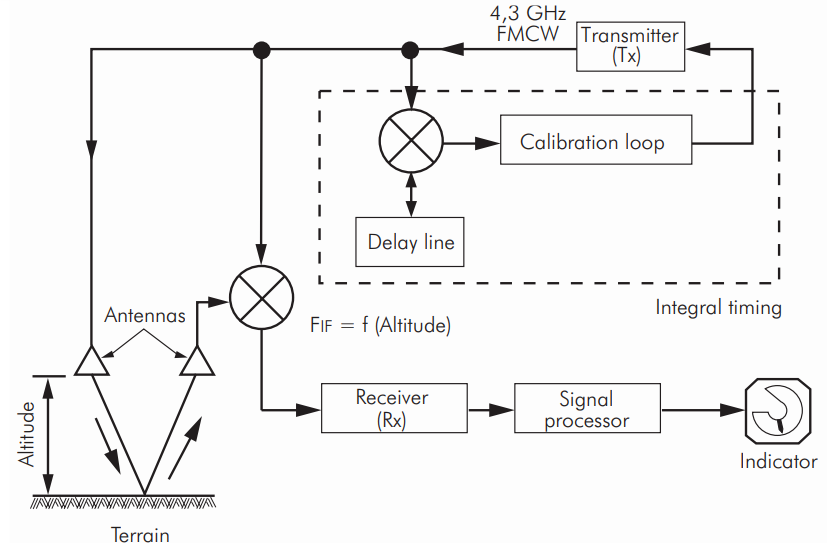
\includegraphics[scale=0.3]{./img/FMCW.png}
	\caption{Esquema del sistema}
\end{figure}

En aquest tipus de sistemes, típicament la modulació en freqüència es produeix per un oscil·lador controlat per voltatge (VCO) que opera a una freqüència central d'aproximadament 4300 MHz amb una estabilitat típica de $\pm 25$ MHz en un rang entre -55 i 70 graus.
Es tracta d'un sistema homodí i la mateixa freqüència de transmissió s'empra com a base de l'oscil·lador local que directament passa la senyal rebuda a banda base després del mixer.

La informació està continguda en la freqüència del senyal que arriba, sent aquesta funció de l'alçada. Així, s'amplifica i  es descodifica   per un bloc de processat de senyal, per exemple. Aquest ha de realitzar una simple operació i traduir el resultat en nivells de voltatge que proporcionarà directament a l'indicador d'alçada de l'aeronau.
\begin{equation}
\label{h1}
H=\frac{c\Delta t}{2}=\frac{c\Delta f}{2\frac{df}{dt}}
\end{equation}
\begin{figure}[H]
	\centering
	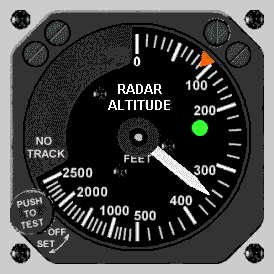
\includegraphics[scale=0.4]{./img/panel}
	\caption{Indicador del radioaltímetre}
\end{figure}
\subsection{Altímetre basat en emissió de polsos}
Generalment, aquesta versió solament necessita una antena doncs funciona com un radar primari  per tant treballa a la mateixa freqüència. Probablement empri un circulador per separar les comunicacions. Es diferencia amb l'anterior cas en el fet que utilitza el $\Delta t$ produït entre el moment d'enviar el pols i el moment de la rebuda, per així determinar l'alçada a la que es troba l'avió. Senzillament, caldria aplicar la primera part de la fórmula de l'eq. \ref{h1}.

\subsection{Antena}
S'ha de tenir en compte  que l'avió rota amb angles de guinyada, capcineig i balanceig. Així doncs, l'antena no ha de ser gaire direccional si no es vol veure afectada per aquestes rotacions. Típicament s'utilitzen antenes que donen entre 8 i 13 dBi de guany i entre 35 i 60 graus del feix d'amplada amb una polarització lineal horitzontal amb un diagrama de radiació cònic.

\subsection{Redundància}
La banda 4200 - 4400 MHz està reservada per aplicacions de radionavegació aeronàutica. Tot i així, s'ha de vigilar força perquè l'antena apunta cap al terra i això fa el sistema més vulnerable. En cas de captar una interferència el radio altímetre podria mesurar una alçada incorrecta. A més, aquest sistema es emprat per altres de forma indirecta, com el TCAS o inclús els \textit{Flight Controls} i per això pot resultar crític.
Per evitar aquest tipus de problemes, moltes aeronaus instal·len fins a tres sistemes de radio altímetres. Ara però, per evitar que es distorsionin mútuament cada emissor treballa amb un offset. Concretament, si hi ha dos sistemes l'\textit{offset} de la freqüència central serà de 5MHz i de 10MHz si es treballa amb tres sistemes.

\subsection{Ample de Banda}
L'ample de Banda disponible és de 200MHz. Alguns sistemes l'utilitzen al complet doncs apliquen tècniques especials per aconseguir valors de precisió molt bons. Quant menys BW utilitzi un sistema, en general serà menys precís. Certament, per un sistema tan rellevant com aquest, què es emprat per altres sistemes com pel sistema de control de vol en períodes d'aproximació i aterratge, la precisió és crucial.

A continuació es presenten els valors de rendiment desitjats d'un sistema d'aquest tipus:
\begin{table}[H]
	\centering
	\begin{tabular}{lc}
		\toprule[3pt]
		\textbf{Alçada}&\textbf{Precisió}\\
		\midrule[1pt]
		0-150m & $\pm$ 2\% de l'alçada \\
		>150m & 5 \% de l'alçada \\
		\bottomrule[2pt]
	\end{tabular}
	\label{C}
	\caption{Rendiment esperat}
\end{table}